\section{Methods}
In this section, we report the results of multiple methods we tried for feature extraction, dimension reduction, and classification. 

\subsection{Data Preprocessing}
\subsubsection{Stemming and Stop Words}
Conclusion: Did not work!

\subsection{Feature Selection}
To extract features from the raw word and image features, we experimented with multiple feature selection methods, including Information Gain, BNS
\subsubsection{Information Gain Over Words Features}
words visualization
\subsection{Dimension Reduction}
\subsubsection{PCA}

\subsection{Classification on Words Features and Extracted Image Features}
\subsubsection{Linear Regression (L2 Regularization) + Sigmoid}
\subsubsection{Logistic Regression + PCA}
\subsubsection{Logistic Regression on Raw Features}
\subsubsection{Naive Bayes}
\subsubsection{Neural Network}
\subsubsection{LogitBoost}
\subsubsection{Kernel SVM}
\subsection{Classification on Image Features}
\subsubsection{Grey-scale Images}
We first convert the profile images data into R, G, B and Grey-scale images. 
\subsubsection{Face Detection with Viola-Jones Algorithm}
We extracted all the faces. We used matlab built-in Viola-Jones algorithm to do face detection on RGB images, which detected faces on 72\% of the profile pictures. All the following classifications over images were based on the faces detected. Later when ensemble, we only used samples with detected faces. For those samples without faces in them, we just set the output of the classifier as 0 (the output of the classifier is either positive or negative for male or female).
\subsubsection{Logistic Regression with Eigen Faces}
After extracted faces, we did PCA over grey-scale images, the visualization of the top principal components are shown in figure below. We put top PCs into logistic regression classifier and it yielded 60+\% accuracy. \\
\begin{center}
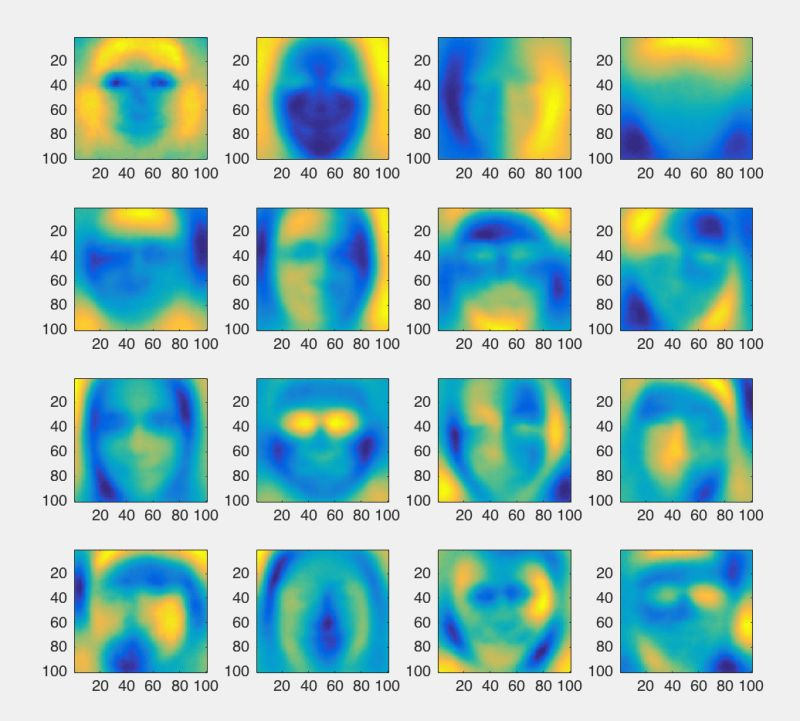
\includegraphics[scale=0.5]{pca_faces}
\end{center}
\subsubsection{SVM on PCA-ed HOG Features}
\subsubsection{SVM on PCA-ed LBP Features}
\subsubsection{Bagging Logistic Regression on PCA-ed HOG Features}
\subsection{Ensemble Methods}
\subsubsection{Stacking}
We used stacking to ensemble our models to achieve better over all performance than any of the single models. First, we used 80\% of the training data to train all the single models including logistic regression, neural network, logitboost with feature selection, kernel SVM with feature selection, kernel SVM with normalization, SVM over PCA-ed HOG, SVM over PCA-ed LBP. And then, use those models to generate predictions (scores) for the rest 20\% data. Training a logistic regression model using the 20\% scores with labels yields a ensemble classifier. Finally, we use all the training data to re-train all the single models. Along with the ensemble classifier, we got our final model. Our full model yielded 92.42\% prediction accuracy on the leaderboard over test set. For the final submission, due to the space and time constraints, we dropped the LBP model and replaced the SVM over PCA-ed HOG with bagging logistic regression over raw HOG features. This final submission yielded 91.04\% prediction accuracy on validation set, ranked 6th.
\subsubsection{Normalization}
When ensemble all the models, we notices that normalization actually works. For the images, we first trained logistic regression on raw gaussian pyramid HOG features (faces, eyes and nose), which yielded 82\% accuracy on detected faces by itself. Later, we figured SVM works better by experiment (84\%). However, when we ensemble the new model, it actually produced lower accuracy. We then found that the scores ranges produced by logistic regression and SVM were actually different. This may cause unbalanced weights across models. We then normalized all the scores with a sigmoid function with mean 0 and variance 2. This produced higher overall accuracy (92.3\%). Tweaking the sigmoid function parameters for each model may produce a little bit higher accuracy but we didn't get enough time for that.
\subsubsection{Cascaded Ensembling}


